\documentclass{article}

\usepackage{tikz}
\usepackage{caption}
\usepackage{subcaption}
\usepackage{pgfplots}
\usepackage{amsmath}
\usepackage{dsfont}
\usepackage{eurosym}
\usepackage{multicol}
\usepackage{abstract}
\usepackage{parskip}
\usepackage{booktabs}
\usepackage{csvsimple}
\usepackage{pdflscape}
\usepackage[pass]{geometry}
\usepackage{lineno,hyperref}

\usepgfplotslibrary{dateplot}

\definecolor{awesomePurple}{rgb}{0.55, 0.42, 1}

\newtheorem{hyp}{Hypothesis}
\newtheorem{alg}{Algorithm}

\newcommand{\W}{\mathcal{W}}
\newcommand{\Lin}{\mathcal{L}}
\newcommand{\G}{\mathcal{G}}
\newcommand{\N}{\mathcal{N}}
\newcommand{\diff}{\textnormal{d}}
\newcommand{\Proba}{\textnormal{Proba}}
\newcommand{\Var}{\textnormal{Var}}

\makeatletter % https://tex.stackexchange.com/a/205193/156344
\newcommand*\short[1]{\expandafter\@gobbletwo\number\numexpr#1\relax}
\makeatother

\geometry{margin=1cm}

\pgfplotsset{colormap/viridis}

\begin{document}

\newgeometry{margin=2cm}

\setlength{\parindent}{0pt}

\title{\huge Pension management \\ \Large Case of a single risky asset and a fixed pension coupon}

\author{Gil-Arnaud Coche}

\maketitle

\begin{abstract}
In this document, a methodology based on Monte-Carlo simulations is presented to compute an optimal investment strategy for the pension self-investor. 
\end{abstract}

At instant $k = 0$, a financial investor has a wealth $\W_0$ from which he wants to be able to receive a pension $c$ at equally spaced instants $k=0\dots K-1$ (\textit{e.g.} monthly). He asks himself what a smart investment strategy would be knowing that he can invest at each instant an amount $\psi_k$ in a risky asset of returns
$$
\mu_k = m + \sigma\epsilon_k\ \ \ \ \epsilon_k\sim\N\left(0, 1\right) \textnormal{ i.i.d.}
$$
and an amount $\psi^0_k$ a riskless asset of returns $r$. Figure \ref{fig:two-period-cash-flow-diagram} shows a diagram of the cash flows the investor is trying to optimize.

\begin{figure}[h!]
\centering
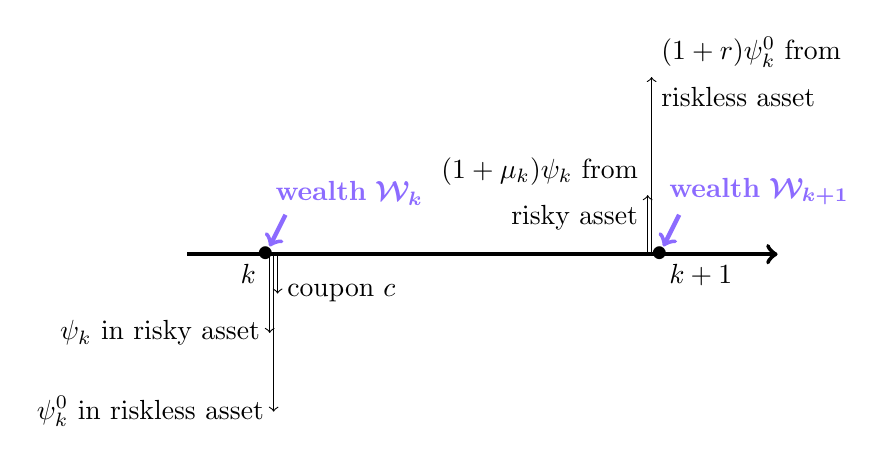
\begin{tikzpicture}[scale = .5]
\draw[->, ultra thick] (-2, 0) -- (13, 0);

\node at (0, 0) {\large $\bullet$};
\node at (0, 0) [below left] {$k$};
\node at (0, 1) [above right] {\color{awesomePurple}\textbf {wealth} $\boldsymbol {\W_{k}}$};
\draw [->, ultra thick, awesomePurple] (.5, 1) -- (0.1, .2);

\node at (10, 0) {\large$\bullet$};
\node at (10, 0) [below right] {$k + 1$};
\node at (10, 1) [above right] {\color{awesomePurple}\textbf {wealth} $\boldsymbol {\W_{k+1}}$};
\draw [->, ultra thick, awesomePurple] (10.5, 1) -- (10.1, .2);

\draw[->] (0.1, 0) -- (0.1, - 2);
\node at (0.1, -2) [left] {$\psi_k$ in risky asset};

\draw[->] (.2, 0) -- (.2, - 4);
\node at (.2, -4) [left] {$\psi^0_k$ in riskless asset};

\draw[->] (.3, 0) -- (.3, - 1);
\node at (.3, -1) [right] {coupon  $c$};


\draw[->] (9.7, 0) -- (9.7, 1.5);
\node at (9.7, 1.5) [above left] {$(1 + \mu_k)\psi_k$ from};
\node at (9.7, 1.5) [below left] {risky asset};

\draw[->] (9.8, 0) -- (9.8, 4.5);
\node at (9.8, 4.5) [above right] {$(1 + r)\psi^0_k$ from};
\node at (9.8, 4.5) [below right] {riskless asset};

\end{tikzpicture}
\caption{Cash flow diagram of a two period investment between instants $k$ et $k + 1$.}
\label{fig:two-period-cash-flow-diagram}
\end{figure}

\section{Wealth dynamics.}

\subsection{Derivation of the recurrence formula}

Between two instants $k$ and $k + 1$, the investor wants to invest $\psi_k$ in the risky asset (without borrowing) and $\psi_k^0$ in the riskless asset after having received a coupon (\textit{i.e.} the pension) $c$ from the portfolio. In mathematical terms, the wealth $\W_k$ is the sum of these three terms positive terms
$$
\W_k = c_k + \psi_k + \psi_k^0 \textnormal{ with } c_k = \min\left(c, \W_k\right).
$$

At instant $(k + 1)^-$ (just before paying himself another coupon and reinvesting), he receives $(1 + \mu_k)\psi_k$ from the risky asset and $(1 + r)\psi_k^0$ from the riskless asset. In mathematical terms, this is written
$$
\W_{k + 1} = (1 + \mu_k)\psi_k + (1 + r)\psi_k^0.
$$

Using these two expressions, we get to
$$
\W_{k + 1} - \left( 1 + r \right)\W_k = \left( \mu_k - r \right)\psi_k - \left( 1 + r \right)c_k
$$
which calls for the definition of actualized to 0 quantities
$$
\tilde \W_k = \frac{\W_k}{\left( 1 + r \right)^k}\ \ \ \ \ \  \tilde\psi_k = \frac{\psi_k}{\left( 1 + r \right)^k}\ \ \ \ \ \  \tilde c_k = \frac{c_k}{\left( 1 + r \right)^k}.
$$

Using these new quantities, we have the following expression
\begin{equation}\label{eq:recurrence-actualized}
\tilde\W_{k + 1} - \tilde\W_k = \frac{\mu_k - r }{1 + r}\tilde\psi_k - \tilde c_k
\end{equation}

\subsection{Derivation of the final wealth formula}

From the previous equation we can derive the wealth at maturity using a telescopic series argument
\begin{equation}
\tilde\W_{K} = \W_0 + \sum_{k = 0}^{K-1} \frac{\mu_k - r }{1 + r}\tilde\psi_k - \sum_{k = 0}^{K-1}\tilde c_k.
\end{equation}

This term shows that the final wealth is the sum of the intial wealth plus the variations from the risky asset investments minus the coupons the investor received at every time step. It suggests the following question: for a given of accetable risk to the investor, it is possible to increase the accessible wealth by investing in the risky asset. Therefore it should be possible to increase the coupon's value, assuming a level of risk aversion, by benefitting from positive trends of a risky asset.

Before moving on to the risk management part of this paper, it is useful to define a benchmark to ``beat'' with the risky investments. What better benchmark than the coupon an completely-risk averse investor would have with a riskless asset only?

\subsection{Riskless linear benchmark.}

In the context of a riskless investment, only investments in the riskless asset are made. In this context, the coupon's delivered at each time step decrease the wealth by the same amount and eventually, the total wealth reaches zero, \textit{i.e.} $\tilde W_K = 0$. The value of the coupon is thus in a closed formula with the maturity. Calling $c_l$ such coupon, we have
$$
 \W_0 = \left( 1 + \frac{1}{r} \right)\left( 1 - \frac{1}{\left( 1 + r \right)^K} \right)c_l.
$$
The naive strategy thus allows a coupon of
\begin{equation}
c_l = \frac{r}{1 + r} \frac{\left( 1 + r \right)^K}{\left( 1 + r \right)^K - 1}  \W_0.
\end{equation}
In the following, this coupon is referred to as the linear benchmark. Note that the term  ``linear'' comes from the limit  $r\ll 1$ where 
$$
\frac{r}{1 + r} \frac{\left( 1 + r \right)^K}{\left( 1 + r \right)^K - 1} \sim \frac{1}{K}
$$
which is the expected coupon without any interest rates.

\section{Strategy and risk management.}

\subsection{Controlling the risk taken by the investor at each period.}

At each period, the investor wants to control the risk he is taking using probabilistic considerations. A simple risk measure is the probability of loss above a threshold. Say that the wealth $\W_k$ at instant $k$ was not invested in the risky asset. Then at $k + 1$, the investor would have $(1+ r)(W_k - c)$.\\

The investor accepts to hold a risky position to beat this amount but refuses that his loss exceeds a fraction of this riskless amount with a probability level. Explicitly, say they do not wish to loose a fraction $\rho$ of the riskless gain $(1+ r)(W_k - c)$ with a probability superior to $\alpha$. This is the same as writing
\begin{equation}
\Proba\left[ \tilde W_{k+1}  \leq \left( 1 - \rho \right) \left( \tilde W_k - \tilde c_k\right) \right] \leq \alpha
\end{equation}

Using \eqref{eq:recurrence-actualized} and assuming that the Sharpe ratio of the risky investment is such that\footnote{In the case where the Sharpe ratio is bigger than $\N^{-1}\left( 1 - \alpha \right)$, then all the remaining capital can be put in the risky asset.} 
$$
\frac{m - r}{\sigma}\leq \N^{-1}\left(1 - \alpha\right)
$$
where $\N^{-1}$ is the inverse of the cumulative normal distribution function, we find after some algebra that the amount invested in risky asset must satisfy
$$
\tilde\psi_k \leq \frac{\rho}{\rho_{\max}} \left( \tilde\W_k - \tilde c_k \right).
$$
with 
\begin{equation}\label{eq:risk-inequality}
\rho_{\max} = \frac{1}{1 + r}\left[ \N^{-1}\left( 1 - \alpha \right) - \frac{m - r}{\sigma} \right].
\end{equation}

\subsection{Investment strategy.}

The previous formula was an inequality. However this inequality may be switched to an equal sign if the investor wishes to maximize its returns between two instants $k$ and $k + 1$. In layman's terms, they choose an optimal portfolio using a Value at Risk type risk measure.

As the investor cannot borrow money to conduct their strategy, they necessarily are capped in the amount they can invest in the risky asset. The maximum amount they can invest is $\tilde\W_k - \tilde c_k$. And therefore,
\begin{equation}\label{eq:no-borrowing-inequality}
\tilde\psi_k\leq \tilde W_k - \tilde c_k.
\end{equation}

The risk management inequality \eqref{eq:risk-inequality} and the no-borrowing condition \eqref{eq:no-borrowing-inequality} suggest to define the following strategy for the investor
\begin{equation}\label{eq:investment-strategy}
\tilde\psi_k = f(\rho) \left(\tilde\W_k - \tilde c_k\right) \textnormal{ with } f(\rho) = \min\left( 1,  \frac{\rho}{\rho_{\max}} \right)
\end{equation}
with $$\rho_{\max} = \frac{1}{1 + r}\left[ \N^{-1}\left( 1 - \alpha \right) - \frac{m - r}{\sigma} \right].$$

\section{Finding an eligible coupon for a less risk averse investor.}

\subsection{Uncertainty of the maturity.}

As the risky asset is subject to random fluctuations, strategically investing in it gives rise to the possibility of ending earlier the investment, or in best case scenarios, later. Nonetheless, in the context of pension funds, it would be wise to be able to have a little control over the end of the investment. Indeed, these types of investor could benefit from extra money while they are alive but also need to receive a coupon for as long as possible.

To provide answers to these questions, we can choose two simple termination conditions to find the coupon value for a risk aversion factor:
\begin{itemize}
\item imposing an average value of zero for the final wealth $\tilde\W_K$ at a desired maturity $K$; calling $\tilde\omega_K(c, \rho)$ the average wealth after $K$ iterations, the investor chooses the value $c(\rho)$ such that
\begin{equation}\label{eq:average-zero-final-wealth}
\tilde\omega_K(c(\rho), \rho) = 0
\end{equation}
\item imposing an average value of $K$ to the life span of the investment; calling $\kappa(c, \rho)$ the life span of an investment with a coupon $c$ and a risk aversion factor $\rho$, the investor chooses to the value $c(\rho)$ such that
\begin{equation}\label{eq:average-K-maturity}
\kappa(c(\rho), \rho)= K.
\end{equation}
\end{itemize}

\subsection{Full statement of the problem.}

The recurrence \eqref{eq:recurrence-actualized}, the termination conditions \eqref{eq:average-zero-final-wealth} and \eqref{eq:average-K-maturity}, and the strategy \eqref{eq:investment-strategy} lead to the inverse problem 
\begin{equation}\label{eq:final-coupon-inverse-formula}
\begin{split}
\tilde\omega_K(c(\rho), \rho) = 0 \textnormal{ or } \kappa(c(\rho), \rho)= K
\end{split}
\end{equation}
with the wealth dynamics
\begin{equation}
\begin{split}
\tilde \W_0 & = \W_0\\
\tilde\W_{k + 1} &= \left( 1 + f(\rho)\frac{\mu_k - r }{1 + r} \right)\left(\tilde\W_k - \min \left[ \frac{c}{\left(1 + r\right)^k}, \tilde\W_k \right]\right)\\
\mu_k & = m + \sigma \epsilon_k\\
\epsilon_k&\sim\N\left(0, 1\right) \textnormal{ i.i.d.}
\end{split}
\end{equation}
and the parameters
\begin{equation}
\begin{split}
f(\rho) &= \min\left( 1, \frac{\rho}{\rho_{\max}} \right)\\
\rho_{\max} &= \frac{1}{1 + r}\left[ \N^{-1}\left( 1 - \alpha \right) - \frac{m - r}{\sigma} \right]
\end{split}
\end{equation}
assuming that the Sharpe ratio of the risky asset is smaller than $\N^{-1}\left( 1 - \alpha  \right)$.

\section{Monte-Carlo Simulation.}

\subsection{Dimensionless wealth dynamics problem}

If we introduce $$\xi = \frac{\rho}{\rho_{\max}}$$ and consider an initial wealth $$\W_0 = 1,$$ the dimensionless wealth dynamics\footnote{As all financial values are proportional to $\W_0$, it makes computations easier to ``drop'' the initial wealth by setting it to 1.} is stated as
\begin{equation}
\begin{split}
\tilde \W_0 & = 1\\
\tilde\W_{k + 1} &= \left( 1 + \xi\frac{\mu_k - r }{1 + r} \right)\left(\tilde\W_k - \min \left[ \frac{c}{\left(1 + r\right)^k}, \tilde\W_k \right]\right)\\
\mu_k & = m + \sigma \epsilon_k\\
\epsilon_k&\sim\N\left(0, 1\right) \textnormal{ i.i.d.}
\end{split}
\end{equation}
The dimensionless risk aversion parameter takes its values between $0$ and $1/\rho_{\max}$.

\subsection{Results}

To run simulations, 
\begin{itemize}
\item the risk free rate is set at $r = 0.005/12$ which is the \href{https://www.capital.fr/votre-argent/livret-a-ldds-lep-cel-pee-les-nouveaux-taux-de-votre-epargne-reglementee-au-1er-fevrier-2020-1361121#:~:text=Livret%20A%20%3A%20taux%20%C3%A0%200%2C5%25&text=Pour%20une%20personne%20l'ayant,de%20115%20euros%20par%20an.}{\color{awesomePurple}livret A rate},
\item we consider that the maturity $K = 24$ which is equivalent to two years,
\item the number of samples in the Monte-Carlo simulations is $S = 100000$, and finally
\item the risky asset is the \href{https://www.abcbourse.com/download/valeur/CACp}{\color{awesomePurple}Lyxor ETF CAC 40} for which monthly data gives $m = 0.02592$ and $\sigma = 0.06164$ from $1^\textnormal{st}$ April 2020 to $31^\textnormal{st}$ March 2021.
\end{itemize}

For these parameter values, we find that 
$
\rho_{\max} = 1.2941
$ which caps the value of $\xi$ to $0.77276$. Figures \ref{fig:fixed-maturity} and \ref{fig:variable-maturity} show the results for $\tilde\omega_K(c(\rho), \rho) = 0$ and $\kappa(c(\rho), \rho)= K$ respectively. 


\begin{figure}[b!]
     \centering
     \hfill
     \begin{subfigure}[b]{\textwidth}
         \centering
         \includegraphics[scale=.7]{png/average_life_span_W0=1_r=0.0004166666666666667_m=0.02592451988463669_sigma=0.06164058158266796_K=24_S=100000.png}
         \caption{}
         \label{fig:average-final-wealth-zero-life-span}
     \end{subfigure}
     \\
     \begin{subfigure}[b]{\textwidth}
         \centering
         \includegraphics[scale=.7]{png/additional_wealth_W0=1_r=0.0004166666666666667_m=0.02592451988463669_sigma=0.06164058158266796_K=24_S=100000.png}
         \caption{}
         \label{fig:average-final-wealth-zero-additional wealth}
     \end{subfigure}
     \\
     \begin{subfigure}[b]{\textwidth}
         \centering
         \includegraphics[scale=.7]{png/expected_shortfall_W0=1_r=0.0004166666666666667_m=0.02592451988463669_sigma=0.06164058158266796_K=24_S=100000.png}
         \caption{}
         \label{fig:average-final-wealth-zero-expected-shortfall}
     \end{subfigure}
        \caption{Imposing a zero average at maturity $K$}
        \label{fig:fixed-maturity}
\end{figure}

\begin{figure}[b!]
     \centering
     \hfill
     \begin{subfigure}[b]{\textwidth}
         \centering
         \includegraphics[scale=.7]{png/average_life_span_non_fixed_W0=1_r=0.0004166666666666667_m=0.02592451988463669_sigma=0.06164058158266796_K=24_S=100000.png}
         \caption{}
         \label{fig:average-final-wealth-zero-life-span}
     \end{subfigure}
     \\
     \begin{subfigure}[b]{\textwidth}
         \centering
         \includegraphics[scale=.7]{png/additional_wealth_non_fixed_W0=1_r=0.0004166666666666667_m=0.02592451988463669_sigma=0.06164058158266796_K=24_S=100000.png}
         \caption{}
         \label{fig:average-final-wealth-zero-additional wealth}
     \end{subfigure}
     \\
     \begin{subfigure}[b]{\textwidth}
         \centering
         \includegraphics[scale=.7]{png/expected_shortfall_non_fixed_W0=1_r=0.0004166666666666667_m=0.02592451988463669_sigma=0.06164058158266796_K=24_S=100000.png}
         \caption{}
         \label{fig:average-final-wealth-zero-expected-shortfall}
     \end{subfigure}
        \caption{Imposing a zero average at maturity $K$}
        \label{fig:variable-maturity}
\end{figure}

As expected, when fixing the average wealth to zero at maturity, the average life span decreases with the decrease of the risk aversion (when $\xi$ increases). This is because imposing an average to zero actually imposes that all value are zero. The wealth is a positive number so \textit{de facto}, the coupon value that cancels it forces the investment to stop earlier. And this early stopping starts as soon as fourteen months for risk taking investors. Also, as expected the potential wealth gain can be significant with an average of $10\%$ for risk takers and up too over $20\%$ for the luckiest of them. However, increased risk also means increased potential losses. And despite the rather high value of the trend ($m = 2.5\%$ per month!), the expected shortfall at $5\%$ can be up to $12\%$ for the least lucky of investors.

When matching the expected maturity, two differences:
\begin{itemize}
\item the average life span remains at 24 months  as expected and the standard deviation of this life span notably increases with risk as there are up to 4 months of uncertainty for the most risky investors. 
\item The increased average life span increases the potential gains while decreasing the potential losses, this is a mechanical effect due to the longer life spans: as the trend is rather high, the odds of loss decrease with time while positive outlooks increase.
\end{itemize}

\section{Wrapping Up}

This short document demonstrate that with a precise strategy and wealth manegement, an investor can determine how they can gain from investing in ETFs. This study assumes rather simple market dynamics hypothesis, however, the general framework provides an acurate methodology to determine optimal pension management.

The model would gain in efficiency if
\begin{itemize}
\item the target average wealth at maturity could be controlled, openning the door to inheritance and transmissions,
\item the returns where modelled with a stochastic volatility model,
\item the random nature of life expectancy was added,
\item multiple risky assets where considered in the portfolio,
\item the wealth dynamic was not computed with discounted values as they bring about underflows,
\item the root finding algorithm used were optimized.
\end{itemize}


Finally, it could be interesting to run a backtesting scenario on multiple ETFs and see for different periods what the risks are.

\end{document}